\documentclass[a4 paper]{article}
% Set target color model to RGB
\usepackage[inner=2.0cm,outer=2.0cm,top=2.5cm,bottom=2.5cm]{geometry}
\usepackage{setspace}
\usepackage[rgb]{xcolor}
\usepackage{verbatim}
\usepackage{subcaption}
\usepackage{amsgen,amsmath,amstext,amsbsy,amsopn,tikz,amssymb,tkz-linknodes}
\usepackage{fancyhdr}
\usepackage[colorlinks=true, urlcolor=blue,  linkcolor=blue, citecolor=blue]{hyperref}
\usepackage[colorinlistoftodos]{todonotes}
\usepackage{rotating}
\usepackage{color}
\usepackage[version=4]{mhchem}
\usepackage[section]{placeins}
\usepackage{float}
\usepackage[justification=centering]{caption}
\usepackage[toc,page]{appendix}

%\usetikzlibrary{through,backgrounds}
\hypersetup{%
pdfauthor={Ashudeep Singh},%
pdftitle={Homework},%
pdfkeywords={Tikz,latex,bootstrap,uncertaintes},%
pdfcreator={PDFLaTeX},%
pdfproducer={PDFLaTeX},%
}
%\usetikzlibrary{shadows}
% \usepackage[francais]{babel}
\usepackage{booktabs}
\newcommand{\ra}[1]{\renewcommand{\arraystretch}{#1}}

\newtheorem{thm}{Theorem}[section]
\newtheorem{prop}[thm]{Proposition}
\newtheorem{lem}[thm]{Lemma}
\newtheorem{cor}[thm]{Corollary}
\newtheorem{defn}[thm]{Definition}
\newtheorem{rem}[thm]{Remark}
\numberwithin{equation}{section}

\newcommand{\homework}[6]{
   \pagestyle{myheadings}
   \thispagestyle{plain}
   \newpage
   \setcounter{page}{1}
   \noindent
   \begin{center}
   \framebox{
      \vbox{\vspace{2mm}
    \hbox to 6.28in { {\bf BIOS611:~Introduction to Data Science \hfill {\small (#2)}} }
       \vspace{6mm}
       \hbox to 6.28in { {\Large \hfill #1  \hfill} }
       \vspace{6mm}
       \hbox to 6.28in { {\it \hfill Instructor: {\rm #3} \hfill } }
       
       \hbox to 6.28in { {\hfill \it Name: {\rm #5}  \hfill #6}}
       %\hbox to 6.28in { {\it TA: #4  \hfill #6}}
      \vspace{2mm}}
   }
   \end{center}
   \markboth{#5 -- #1}{#5 -- #1}
   \vspace*{4mm}
}

\newcommand{\problem}[2]{~\\\fbox{\textbf{Problem #1}}\hfill (#2 points)\newline\newline}
\newcommand{\subproblem}[1]{~\newline\textbf{(#1)}}
\newcommand{\D}{\mathcal{D}}
\newcommand{\Hy}{\mathcal{H}}
\newcommand{\VS}{\textrm{VS}}
\newcommand{\solution}{~\newline\textbf{\textit{(Solution)}} }

\newcommand{\bbF}{\mathbb{F}}
\newcommand{\bbX}{\mathbb{X}}
\newcommand{\bI}{\mathbf{I}}
\newcommand{\bX}{\mathbf{X}}
\newcommand{\bY}{\mathbf{Y}}
\newcommand{\bepsilon}{\boldsymbol{\epsilon}}
\newcommand{\balpha}{\boldsymbol{\alpha}}
\newcommand{\bbeta}{\boldsymbol{\beta}}
\newcommand{\0}{\mathbf{0}}

\begin{document}


\bibliographystyle{unsrt}
\homework{Final Report of BIOS 611}{Time: 12/05/21}{\textit{Prof.} Toups}{}{Yixiang Qu}

\rule{\textwidth}{0.1pt}

\tableofcontents


\section{Introduction}
With progress on both the theoretical and the computational fronts, the use of spline modelling has become an established tool in statistical regression analysis. In particular, splines are regularly used for building explanatory models in clinical research, since irregular time series often occurs in biomedical researches\cite{coenen2020primer}. Indeed, many new methodological developments in modern biostatistics make use of splines to model smooth functions of interest. However, when it comes to very complicated model structure, traditional splines methods may not work well and may not help to make use of all the information. In my first year of my PhD, I made a deep learning tool for better interpolate microbiome data. In order to compare its performance with traditional spline methods, I made this project. It will use Rshiny to show the difference of the interpolation results of my deep learning method and the B-spline method.

\section{The complicated data structure of microbiome time series data}

The time series data two dimensions originally. However, since there are multiply observations of microbiome species at one time point, the dataset has three dimensions, called a multivariate time series dataset.

Consider a $N$-subject time series dataset with $V$-dimensional covariates. We can use $j \in \{1,2,\ldots,N \}$ to denote the $j$-th subject. For the $j$-th subject with $L_j$ samples, we use $\mathbf{T_j} = (t_{j,1}, t_{j,2}, \ldots, t_{j,L_j})$ to denote the observation time points. And for the $i$-th ($i \in\{1,2, \ldots, L_j\}$) time point, the observation values $\mathbf{y_{j,i}}$ will be a $V$-dimensional vector. Therefore, for the $j$-th subject, we can denote the observation values as $\mathbf{Y_j}\in \mathbb{R}^{L_{j}\times V}$. And if there are missing values in the $j$-th subject, we can use mask matrix $\mathbf{M_j}\in\{0,1\}^{L_{j}\times V}$ to indicate the missing information, where 0 indicated that the information is missing at the specific time point for the certain subject.

\begin{table}[h!]
  \centering
  \caption{A example data format of multivariate microbiome time series dataset}
    \begin{tabular}{c|c|c|c|c|c|c|c|c|c}
    ID    & Time  & Value\_1 & Value\_2 & {$\ldots$} & Value\_V & Mask\_1 & Mask\_2 & {$\ldots$} & Mask\_V \\ \midrule
    {1} & $t_{1,1}$ & $y_{1,1,1}$ & $y_{1,1,2}$ &       & $y_{1,1,V}$ & $m_{1,1,1}$ & $m_{1,1,2}$ &       & $m_{1,1,V}$ \\ \hline
    {1} & $t_{1,2}$ & $y_{1,2,1}$ & $y_{1,2,2}$ &       & $y_{1,2,V}$ & $m_{1,2,1}$ & $m_{1,2,2}$ &       & $m_{1,2,V}$ \\ \hline
    {1} & $t_{1,3}$ & $y_{1,3,1}$ & $y_{1,3,2}$ &       & $y_{1,3,V}$ & $m_{1,3,1}$ & $m_{1,3,2}$ &       & $m_{1,3,V}$ \\ \hline
    {2} & $t_{2,1}$ & $y_{2,1,1}$ & $y_{2,1,2}$ &       & $y_{2,1,V}$ & $m_{2,1,1}$ & $m_{2,1,2}$ &       & $m_{2,1,V}$ \\ \hline
    {2} & $t_{2,2}$ & $y_{2,2,1}$ & $y_{2,2,2}$ &       & $y_{2,2,V}$ & $m_{2,2,1}$ & $m_{2,2,2}$ &       & $m_{2,2,V}$ \\ \hline
    $\ldots$ &       &       &       &       &       &       &       &       &  \\ \hline
    j     & $t_{j,1}$ & $y_{j,1,1}$ & $y_{j,1,2}$ &       & $y_{j,1,V}$ & $m_{j,1,1}$ & $m_{j,1,2}$ &       & $m_{j,1,V}$ \\ \hline
    j     & $t_{j,2}$ & $y_{j,2,1}$ & $y_{j,2,2}$ &       & $y_{j,2,V}$ & $m_{j,2,1}$ & $m_{j,2,2}$ &       & $m_{j,2,V}$ \\ \hline
    $\ldots$ &       &       &       &       &       &       &       &       &  \\ \hline
    j     & $t_{j,L_j}$ & $y_{j,L_j,1}$ & $y_{j,L_j,2}$ &       & $y_{j,L_j,V}$ & $m_{j,L_j,1}$ & $m_{j,L_j,2}$ &       & $m_{j,L_j,V}$ \\ \hline
    $\ldots$ &       &       &       &       &       &       &       &       &  \\ \hline
    N     & $t_{N,1}$ & $y_{N,1,1}$ & $y_{N,1,2}$ &       & $y_{N,1,V}$ & $m_{N,1,1}$ & $m_{N,1,2}$ &       & $m_{N,1,V}$ \\ \hline
    N     & $t_{N,2}$ & $y_{N,2,1}$ & $y_{N,2,2}$ &       & $y_{N,2,V}$ & $m_{N,2,1}$ & $m_{N,2,2}$ &       & $m_{N,2,V}$ \\ \hline
    N     & $t_{N,3}$ & $y_{N,3,1}$ & $y_{N,3,2}$ &       & $y_{N,3,V}$ & $m_{N,3,1}$ & $m_{N,3,2}$ &       & $m_{N,3,V}$ \\ 
    \end{tabular}
\label{input_format}
\end{table}

\section{Interpolation results of different spline methods}

\subsection{Deep learning interpolation}\label{sec3}

The model to interpolate the time series data is related to my paper, which is under preperation, so I apologize that I cannot write too much details in the report. A concise diagram is shown as Fig. \ref{diagram}.

\begin{figure}[ht]
    \centering
    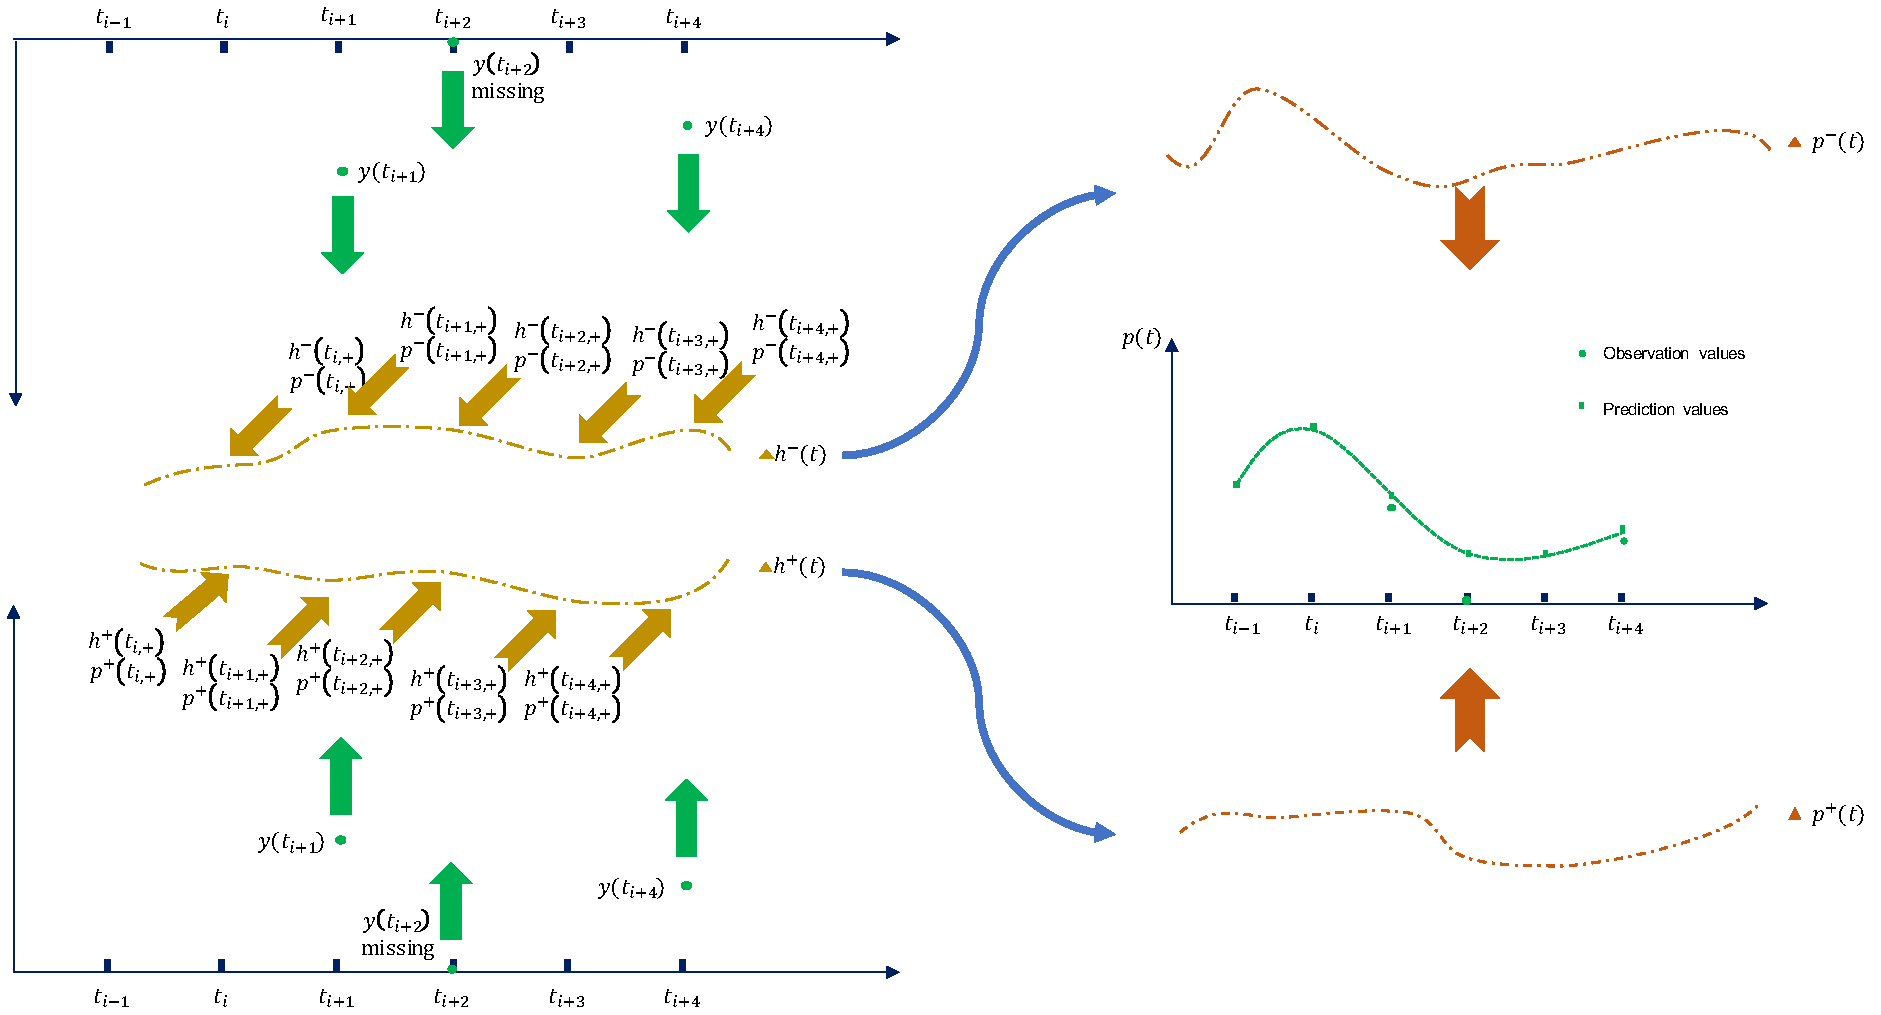
\includegraphics[width=0.9\textwidth]{picture/gruode_model.pdf}
    \caption{A concise diagram of deep learning model}
    \label{diagram}
    \end{figure}

There are two procedures to use deep learning method to interpolate the data.

\begin{enumerate}
    \item Feed all data into the model, and learn the time trend using the deep learning model.
    \item Use the tuned-parameter model to interpolate the data.
\end{enumerate}

I used Pytorch\cite{NEURIPS2019_9015} to implement the deep learning model. And the interpolation results of deep learning model is shown in Fig. \ref{dl}.

\begin{figure}[ht]
    \centering
    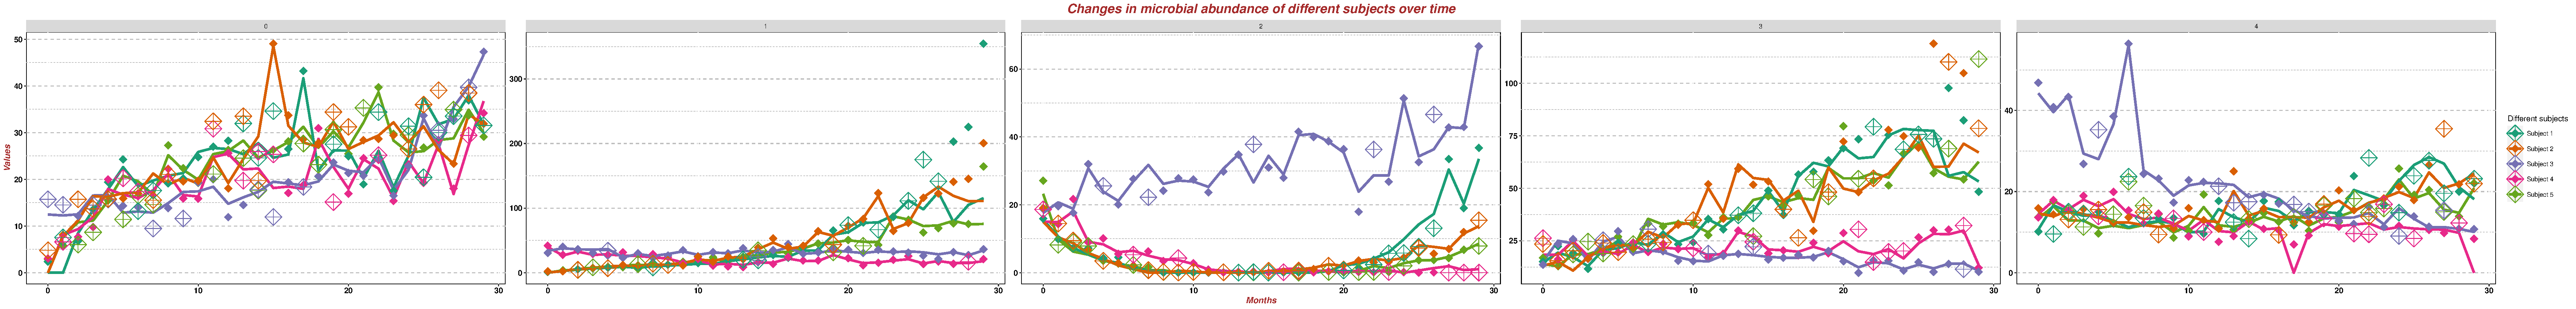
\includegraphics[width=0.9\textwidth]{figure/DL_spline.pdf}
    \caption{Results of deep learning interpolation.\\The information shown in solid points are used to train the model. However, the rest information was not used for the training process.}
    \label{dl}
\end{figure}

\subsection{B spline interpolation}

B-spline is widely used in nonparametric models in biomedical data. B-splines can be defined by construction by means of the Cox-de Boor recursion formula. Given a knot sequence $\ldots, t_{0}, t_{1}, t_{2}, \ldots$, then the Bsplines of order 1 are defined by Eq. \ref{BS_1}.

\begin{equation}
\label{BS_1}
    B_{i, 1}(x):= \begin{cases}1 & \text { if } \quad t_{i} \leq x<t_{i+1} \\ 0 & \text { otherwise }\end{cases}
    \end{equation}
    
These satisfy $\sum_{i} B_{i, 1}(x)=1$ for all $x$ because for any $x$ exactly one of the $B_{i, 1}(x)=1$, and all the others are zero.
The higher order B-splines are defined by recursion, shown in Eq. \ref{BS_3} and Eq. \ref{BS_2}.

\begin{gather}
\omega_{i, k}(x):= \begin{cases}\frac{x-t_{i}}{t_{i+k}-t_{i}}, & t_{i+k} \neq t_{i} \\ 0, & \text { otherwise }\end{cases}\label{BS_3}\\
B_{i, k+1}(x):=\omega_{i, k}(x) B_{i, k}(x)+\left[1-\omega_{i+1, k}(x)\right] B_{i+1, k}(x)\label{BS_2}
\end{gather}

I use gam\cite{gam} to do the B-spline interpolation. And the interpolation results of B-spline model is shown in Fig. \ref{bs}.

\begin{figure}[ht]
    \centering
    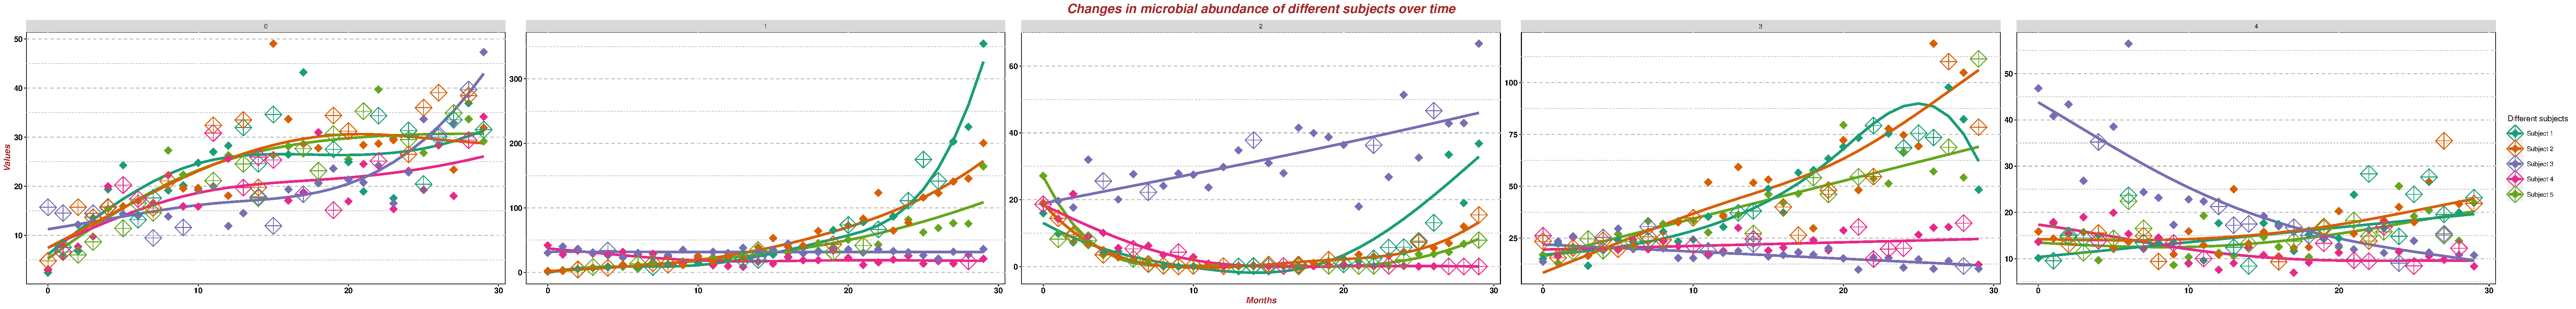
\includegraphics[width=0.9\textwidth]{figure/B_spline.pdf}
    \caption{Results of B spline interpolation.\\The information shown in solid points are fed into the spline model. However, the rest information was not used for this process.}
    \label{bs}
\end{figure}


\subsection{Comparsion of the different interpolation methods}

We can find out from Fig. \ref{dl} and Fig. \ref{bs} that the B spline method seems too smooth that it can not represent the fluctuation of microbiome time series. And we use mean difference to compare the interpolation results of different methods, which is shown in Eq. \ref{MD}, and the results are shown in Table \ref{results}.

\begin{equation}
\label{MD}
\text{Mean Difference} =\frac{1}{n} \sum_{i=1}^n|p_i-o_i|    
\end{equation}

\begin{table}[ht]
\centering
\caption{Mean Difference of different interpolation methods}
\begin{tabular}{|c|c|c|}
\hline
                & Deep Learning & B Spline \\ \hline
Mean Difference & 3.205         & 4.039    \\ \hline
\end{tabular}
\label{results}
\end{table}

\section{Conclusion}

From the previous figures and tables, we can see that the deep learning methods perform better in the interpolation task. The main reason for it is that the deep learning method will learn the time trend of all the subjects, and use the learned information to interpolate the results. However, the spline will only use the information of a single subject. However, the deep learning method will cost far more time than spline method. Therefore, we need to decide whether speed or precision should be the priority before choosing the methods.


\addcontentsline{toc}{section}{References}
\bibliography{ref}

\end{document} 

